\begin{landscape}

  \section*{Parse Tree}
  \label{app:parse-tree}
  \addcontentsline{toc}{section}{Parse Tree}
  \begin{figure}[htb!]
    \centering
    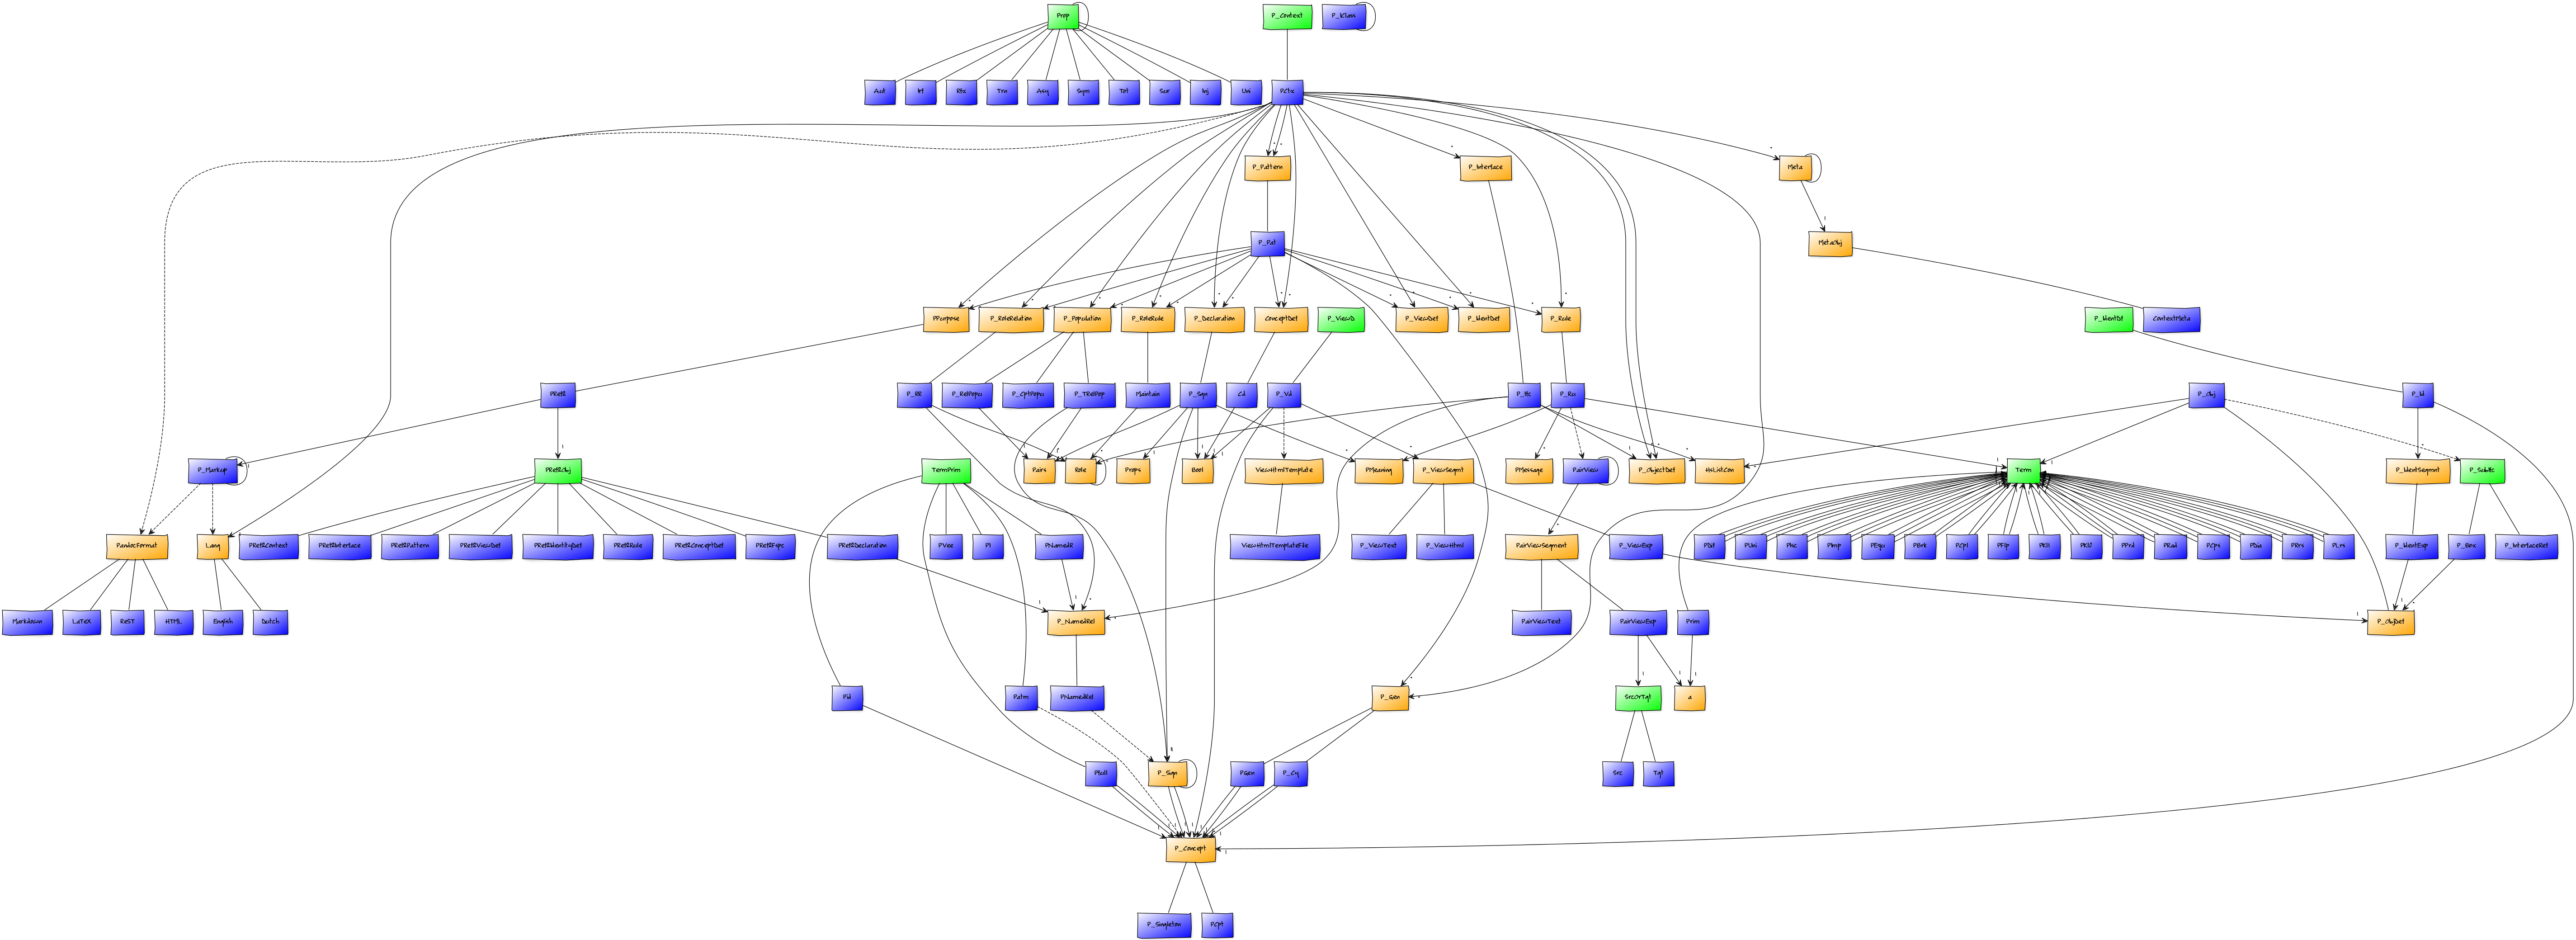
\includegraphics[width=25.4cm]{Figures/GenParseTree}
    \caption{Diagram of the Ampersand parse tree.\small
      %Data definitions are depicted in green, constructors are depicted in blue and 
      Connections without an arrow represent the data contructors.
      Connections with an arrow also show the multiplicity in the relationship (i.e. 1 and *) or are stripped to represent an optional relationship.
      }
    \label{fig:parse-tree}
  \end{figure}

\end{landscape}